\chapter{Tables and Figures}
\label{ch:floats}

\section{Tables}
\label{sec:tables}

The document class includes the ``\verb|booktabs|'' package ---
\url{https://ctan.org/pkg/booktabs} --- for preparing high-quality
tables.

Table captions are placed {\itshape above} the table.

Because tables cannot be split across pages, the best placement for
them is typically the top of the page nearest their initial cite. To
ensure this proper ``floating'' placement of tables, use the environment
\textbf{table} to enclose the table's contents and the table caption.
The contents of the table itself must go in the \textbf{tabular}
environment, to be aligned properly in rows and columns, with the
desired horizontal and vertical rules.

Immediately following this sentence is the point at which
Table~\ref{tab:freq} is included in the input file; compare the
placement of the table here with the table in the printed output of
this document.

\begin{table}[h]
  \centering
  \caption{Frequency of Special Characters}
  \label{tab:freq}
  \begin{tabular}{ccl}
    \toprule
    Non-English or Math&Frequency&Comments\\
    \midrule
    \O & 1 in 1,000& For Swedish names\\
    $\pi$ & 1 in 5& Common in math\\
    \$ & 4 in 5 & Used in business\\
    $\Psi^2_1$ & 1 in 40,000& Unexplained usage\\
    \bottomrule
\end{tabular}
\end{table}

To set a wider table, which takes up the whole width of the page's live
area, use the environment \textbf{table*} to enclose the table's
contents and the table caption. As with a single-column table, this wide
table will ``float'' to a location deemed more desirable. Immediately
following this sentence is the point at which Table~\ref{tab:commands}
is included in the input file; again, it is instructive to compare the
placement of the table here with the table in the printed output of this
document.

\begin{table*}[h]
  \centering
  \caption{Some Typical Commands}
  \label{tab:commands}
  \begin{tabular}{ccl}
    \toprule
    Command &A Number & Comments\\
    \midrule
    \texttt{{\char'134}author} & 100& Author \\
    \texttt{{\char'134}table}& 300 & For tables\\
    \texttt{{\char'134}table*}& 400& For wider tables\\
    \bottomrule
  \end{tabular}
\end{table*}

Always use midrule to separate table header rows from data rows, and use
it only for this purpose. This enables assistive technologies to
recognise table headers and support their users in navigating tables
more easily.

\section{Figures}
\label{sec:figures}

The ``\verb|figure|'' environment should be used for figures. One or
more images can be placed within a figure. If your figure contains
third-party material, you must clearly identify it as such, as shown in
the example below.
\begin{figure}[h]
  \centering
 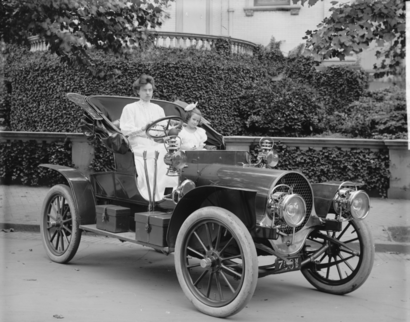
\includegraphics[width=\linewidth]{sample-franklin}
  \caption{1907 Franklin Model D roadster. Photograph by Harris \&
    Ewing, Inc. [Public domain], via Wikimedia
    Commons. (\url{https://goo.gl/VLCRBB}).}
  \Description{A woman and a girl in white dresses sit in an open car.}
\end{figure}

Your figures should contain a caption which describes the figure to the
reader.

Figure captions are placed {\itshape below} the figure.

Every figure should also have a figure description unless it is purely
decorative. These descriptions convey what is in the image to someone
who cannot see it. They are also used by search engine crawlers for
indexing images, and when images cannot be loaded.

A figure description must be unformatted plain text less than 2000
characters long (including spaces). {\bfseries Figure descriptions
  should not repeat the figure caption --- their purpose is to capture
  important information that is not already provided in the caption or
  the main text of the paper.}

\subsection{Full-width Figures}
\label{sec:wide-figures}

An image, or set of images in one figure, that spans the page is created
with the \textbf{figure*} environment, in the same way as a wide table:
\begin{verbatim}
  \begin{figure*}
    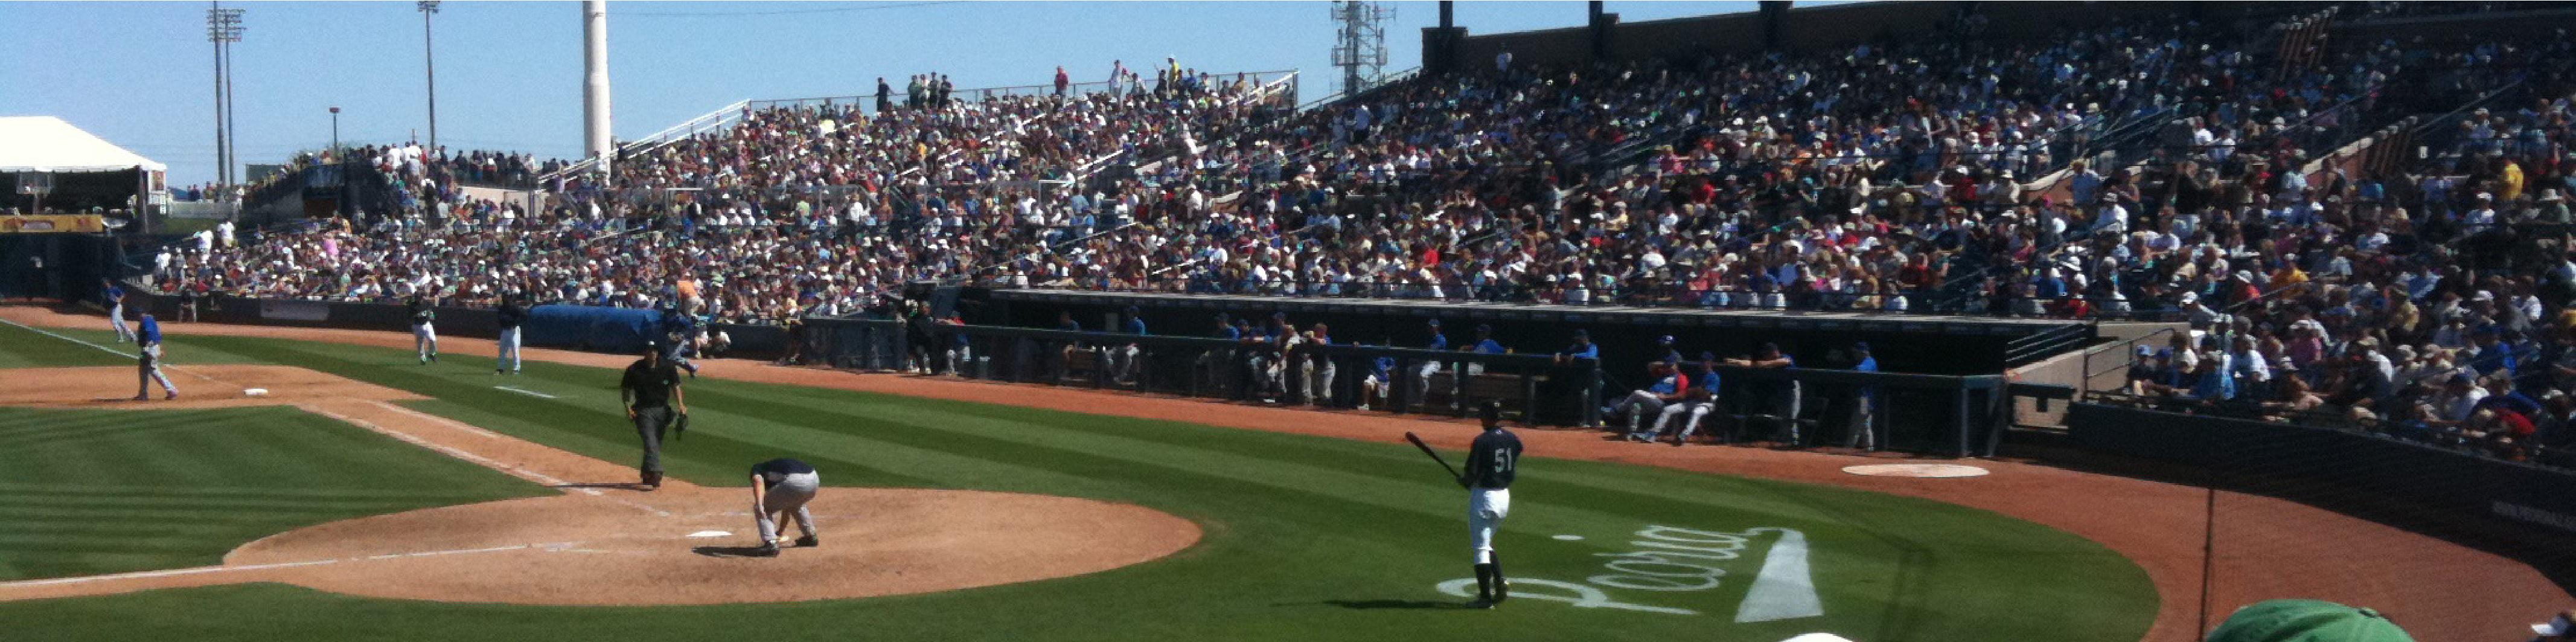
\includegraphics[width=\textwidth]{sampleteaser}
    \caption{figure caption}
    \Description{figure description}
  \end{figure*}
\end{verbatim}

\begin{figure*}
  \centering
  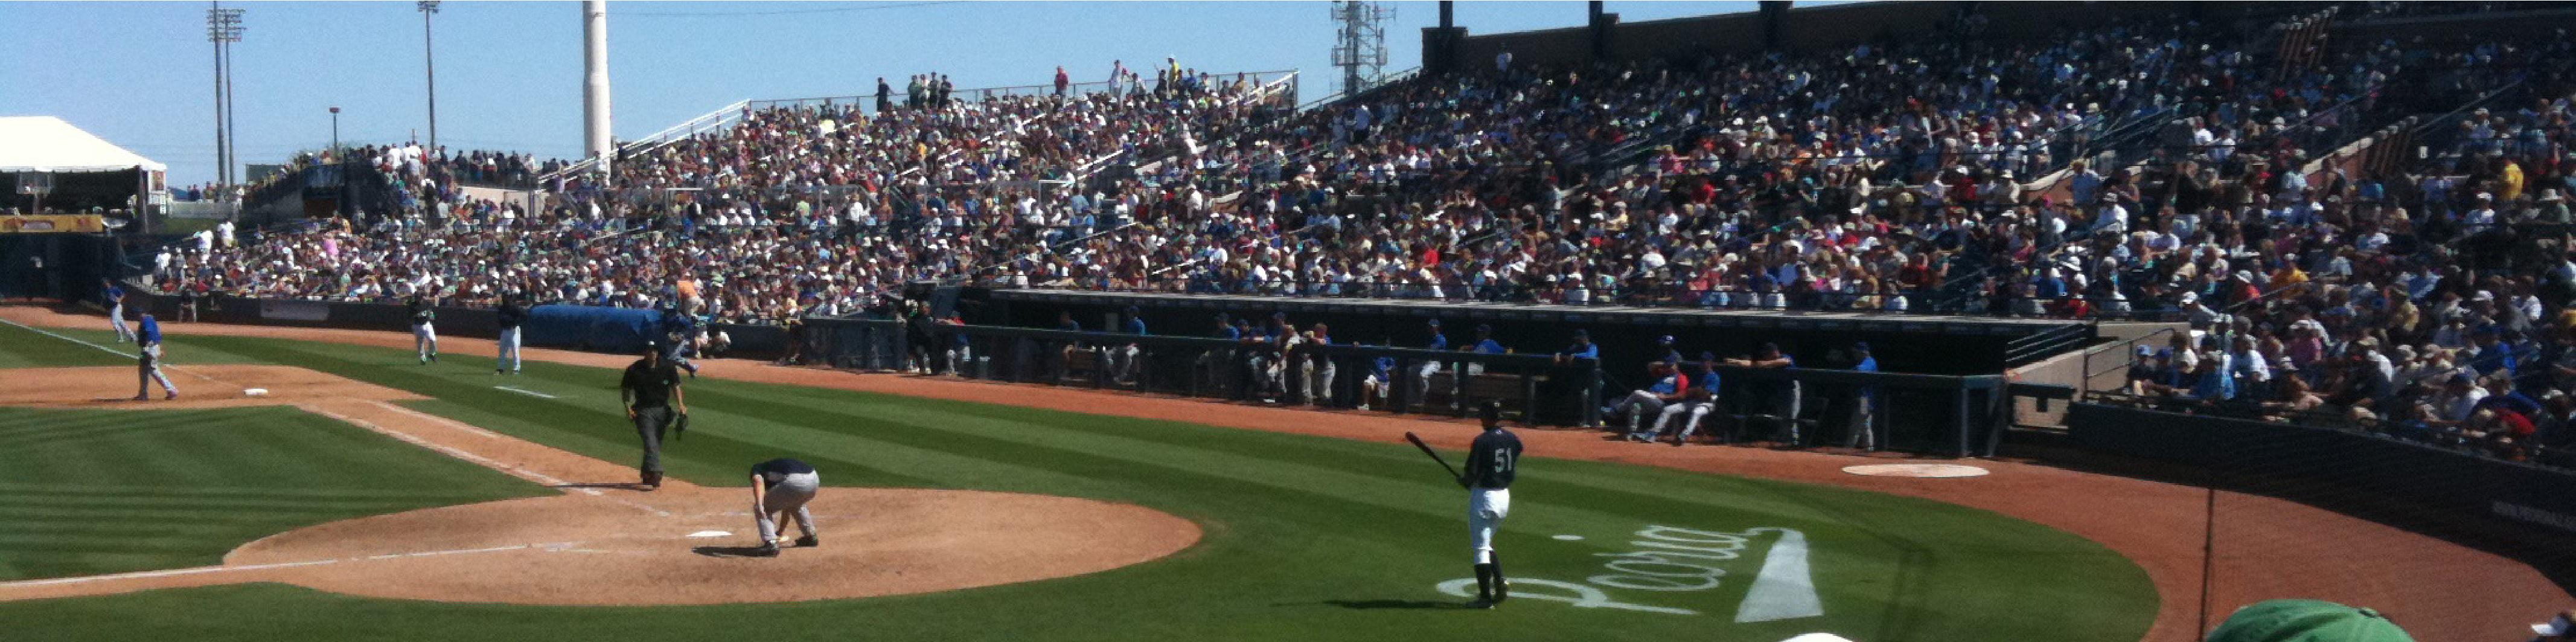
\includegraphics[width=\textwidth]{sampleteaser}
  \caption{Seattle Mariners at Spring Training, 2010.}
  \Description{Enjoying the baseball game from the third-base seats.
    Ichiro Suzuki preparing to bat.}
  \label{fig:teaser}
\end{figure*}
